\documentclass[]{article}
\usepackage[german]{babel}
\usepackage{graphicx}
\usepackage{tabularx}
\usepackage[backend=bibtex, natbib=true]{biblatex}
\usepackage{listings}
\usepackage{tikz}

\lstset{%
	basicstyle=\ttfamily\scriptsize,        % Code font, Examples: \footnotesize, \ttfamily
	keywordstyle=\color{blue!80!black},     % Keywords font ('*' = uppercase)
	commentstyle=\color{gray},              % Comments font
	numbers=left,                           % Line nums position
	numberstyle=\tiny,                      % Line-numbers fonts
	stepnumber=1,                           % Step between two line-numbers
	numbersep=5pt,                          % How far are line-numbers from code
	backgroundcolor=\color{gray!10!white},  % Choose background color
	frame=none,                             % A frame around the code
	tabsize=2,                              % Default tab size
	captionpos=b,                           % Caption-position = bottom
	breaklines=true,                        % Automatic line breaking?
	breakatwhitespace=false,                % Automatic breaks only at whitespace?
	showspaces=false,                       % Dont make spaces visible
	showstringspaces=false                  %
	showtabs=false,                         % Dont make tabls visible
	columns=flexible,                       % Column format
	morekeywords={},                        % Specific keywords
	stringstyle=\color{green!50!black},%
}%

\bibliography{bibliography}
%opening
%Here you can enter your names and titleof your report
\title{Weekly Reports}
\author{Luftqualität in Innenräumen - Gruppe 1}

\begin{document}

\maketitle

\begin{table}[h!]
	\centering
	\begin{tabular}{|c|c|c|}
		\hline
		{\textbf{Name}}				&		{\textbf{Matrikel Nr.}} & {\textbf{Arbeitsaufwand (h)}} \\
		\hline
		Friedrich Just				&		1326699 				&		16,00\\
		\hline
		Stipe Knez					&		1269206 				&	19,00	\\
		\hline
		Lucas Merkert				&		1326709					&	17,00	\\
		\hline
		Achim Glaesmann				&		1309221					&	19,50	\\
		\hline
		Max-Rene Konieczka			&		1211092					&	21,00	\\
		\hline
		Can Cihan Nazlier			&		1179244					&	25,00	\\
		\hline
	\end{tabular}
	\caption{Arbeitsaufwand dieser Woche}
	\label{tab:worakload}
\end{table}



\section{Überblick}


\subsection{Friedrich Just}
Diese Woche wurde die Syntax der Messdaten erneut überarbeitet. Die Sensornamen werden jetzt nicht mehr übertragen. Siehe Abbildung \ref{img:Payload}. Die Übertragung der Daten funktioniert so weit. Sobald der Mikrocontroller an eine Batterie angeschlossen, welche nicht ganz voll ist, kann der Mikrocontroller nicht alle Sensoren normal initialisieren und es werden keine korrekten Werte ausgelesen. Für das korrekte Auslesen der Sensoren muss der Mikrocontroller über die UART-Bridge oder zwei neue Batterien angeschlossen werden. Dies sieht man in der  Abbildung \ref{img:Payload}. Bei dem ersten Datensätze ist die Stromversorgung ausreichend und bei den zweiten reicht diese nicht für alle Sensoren aus.  

\begin{figure}[!h]
	\centering
	\includegraphics[scale=0.40]{images/payload}
	\caption{Messdaten}
	\label{img:Payload}
\end{figure}

\begin{figure}[!h]
	\centering
	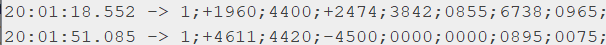
\includegraphics[scale=0.80]{images/UART_fehler}
	\caption{Ausgaben mit Batterie und UART als Stromversorgung}
	\label{img:UART_fehler}
\end{figure}



\subsection{Stipe Knez}
Vergangene Woche war die Hauptaufgabe die Einarbeitung und Vertiefung in die D3.js library. Es ist bereits gelungen einen Prototypen eines Diagramms zu erstellen, das in Zukunft die Daten, die von den ZigBee Modulen empfangen werden, grafisch aufbereitet darstellen soll.
Bei einem persönlichen Treffen der ganzen Gruppe bei Can zuhause wurde das Empfangen realer Daten der ZigBee Module im Backend und das Einspeichern dieser in der Datenbank erfolgreich getestet. Dies geschah bisher nur mit Mock-Daten. Außerdem wurden die zukünftigen Funktionen des Dashboards besprochen und überlegt, ob man verschiedene Messwerte in einem Graphen mit unterschiedlicher Farbe darstellen kann bzw. sollte. Das Treffen in Person ist als sehr erfolgreich zu beurteilen und hat sehr gute Ergebnisee mit sich gebracht.
\subsection{Lucas Merkert}
In dieser Woche ist das Senden der Sensordaten mit mehreren Funkmodulen, welche jeweils alle drei Sensoren angeschlossen hatten gelungen. Die Daten werden über die ZigBee Module (Endgeräte) an den Coordinator geschickt und von diesem über einen COM-Port an die Datenbank gesendet. Allerdings sind dabei noch einige Fehler aufgetreten: In erster Linie wird der Sensor SCD41 manchmal nicht richtig angesprochen. Dies könnte mehrere Gründe haben: Es könnten Falsche Timer gesetzt sein, es könnte einen Fehlerhafter Zustand oder einen fehlerhafte Zustandsübergang geben. Die Ursache dafür soll im Verlauf der nächsten Woche überprüft werden. Außerdem geben die Sensoren sehr unterschiedliche und teilweise unrealistische Werte aus. Hierbei stellt sich die Frage ob es noch Möglichkeiten zur Kalibrierung gibt oder ob die angewendeten Formeln zur Werteberechnung fehlerhaft sind. Auch dies soll noch im Verlauf der kommenden oder der darauffolgenden Woche geklärt werden.


\subsection{Achim Glaesmann}
Diese Woche wurde daran gearbeitet die Verschiedenen Teile der Applikation, bestehend aus Mikrokontroller, deren Firmware, dem Backend so wie dem Frontend zusammenzuführen. Als Schnittstelle zur Applikation wurde der Communication Port des ausführenden Rechners gewählt. Die Sensordaten konnten Erfolgreich als String an das Backend gesendet werden. Hierbei wurde der String wie folgt Designed: IDCONTROLLER;SENSORDATASHT;SENSORDATASCD;SENSORDATACCS;;
Die Kommunikation aller Applikationsbereiche funktionierte erstaunlicherweise direkt mit nur minimalen Fehlern. So erkannte das Backend zum Beispiel das Abschlusszeichen am Ende des Strings der UART-Ausgabe nicht als Whitespace, was Probleme mit der Funktion gab, die Whitespaces entfernte.
 Als einziges nennenswertes Problem ist die Kalibrierung der Sensoren zu nennen, da die Werte hier teilweise noch stark von den Werten abweichen die zu erwarten sind. Dieses Problem kann aber vorraussichtlich in der verbleibenden Zeit behoben werden.Im allgemeinen, gab es also keine unvorhergesehenen Probleme und die verbleibende Zeit kann dazu genzutzt werden die Applikation weiter zu verbessern.


\subsection{Max-Rene Konieczka}
Nach einem Zusammentreffen der Gruppe am 23.01.2022, ist es uns gelungen die eigentlichen Sensordaten in die Datenbank zu übertragen. Da diese nun gespeichert sind, müssen sie nur noch visuell im Dashboard angezeigt werden. Im Verlauf der letzten Woche wurde sich hauptsächlich mit der Einarbeitung in die D3.js-Library beschäftigt. Zunächst wurde lediglich ein einfaches Diagramm erstellt, im nächsten Schritt wird sich um das graphische Anzeigen der Daten gekümmert. Hierbei soll ein Graph erstellt werden, welcher sich in Echtzeit anpasst, abhängig davon in welchem Zeitraum die Daten im Frontend ankommen. Zurzeit werden alle 10 Sekunden Daten im Backend abgespeichert. Es wurde überlegt mehrere Diagramme zu erstellen, um die verschiedenen Sensorwerte besser voneinander unterscheiden zu können.  

\subsection{Can Cihan Nazlier}
Diesen Sonntag gab es ein Treffen mit allen Gruppenmitgliedern bei mir Zuhause. Dort wurde das Zusammenspiel aus Frontend, Backend und den Sensoren mit echten Messwerten getestet. Dieses Treffen lief reibungslos und alle Komponenten haben wie erwartet miteinander kommuniziert. Daran anknüpfend wurden im Frontend Info-Buttons, zu jeweiligen Räumen wo die Sensoren liegen erstellt, die dann Echtzeit-Messdaten der Sensoren im Frontend anzeigen. Das Speichern der Messwerte in die Datenbank klappt auch wie erwartet.
Die Sensoren, die man in die Räume hinzugefügt hat, sind in einer separaten Tabelle in der Datenbank gespeichert, um Positionen der jeweiligen Sensoren nicht zu verlieren.
Der letzte Schritt ist nun das Dashboard zu erstellen.

\printbibliography
%----------------------------------------------------------------------------
% Bibliography
%----------------------------------------------------------------------------	

\end{document}
